\chapter{Konzepte}

\section{Fachliche Strukturen (Domäne)}

\begin{quote}
	Fachliche Modelle, Domänenmodelle, Business-Modelle – sie alle beschreiben Strukturen der reinen Fachlichkeit, also ohne Bezug zur Implementierungs- oder Lösungstechnologie.
	Oftmals tauchen Teile solcher fachlichen Modelle an vielen Stellen in der Architektur, insbesondere der Bausteinsicht, wieder auf. 
	Das "Domain-Driven-Design" oder die uralte "essentielle Systemanalyse" können Ihnen hierbei helfen.
	
	Mit Absicht stellen wir diesen Abschnitt an den Anfang der übergreifenden Konzepte.
\end{quote}

\section{Typische Muster und Strukturen}

\begin{quote}
	Oftmals tauchen einige typische Lösungsstrukturen oder Grundmuster an mehren Stellen der Architektur auf. Beispiele dafür sind die Abhängigkeiten zwischen Persistenzschicht, Applikation sowie die Anbindung grafischer Oberflächen an die Fach- oder Domänenobjekte. Solche wiederkehrenden Strukturen beschreiben Sie möglichst nur ein einziges Mal, um Redundanzen zu vermeiden. Dieser Abschnitt erfüllt genau diesen Zweck.
\end{quote}

\section{Ablaufsteuerung}

\begin{quote}
	Ablaufsteuerung von IT-Systemen bezieht sich sowohl auf die an der (grafischen) Oberfläche sichtbaren Abläufe als auch auf die Steuerung der Hintergrundaktivitäten. Zur Ablaufsteuerung gehört daher unter anderem die Steuerung der Benutzungsoberfläche, die Workflow- oder Geschäftsprozessteuerung sowie Steuerung von Batchabläufen.
\end{quote}

\section{Ausnahme- und Fehlerbehandlung}

\begin{quote}
	Wie werden Programmfehler und Ausnahmen systematisch und konsistent behandelt?
	Wie kann das System nach einem Fehler wieder in einen konsistenten Zustand gelangen? Geschieht dies automatisch oder ist manueller Eingriff erforderlich? Dieser Aspekt hat mit Logging, Protokollierung und Tracing zu tun.
	Welche Art Ausnahmen und Fehler behandelt ihr System? Welche Art Ausnahmen werden an welche Außenschnittstelle weitergeleitet und welche Ausnahmen behandelt das System komplett intern? Wie nutzen Sie die Exception-Handling Mechanismen ihrer Programmiersprache? Verwenden Sie checked- oder unchecked-Exceptions?
\end{quote}

\section{Batchverarbeitung}

\begin{quote}
	Batchverarbeitung sequentielle Verarbeitung einer i.d.R. vorab festgelegten Menge an Daten oder Aufgaben.
\end{quote}

\section{Bedienoberfläche}
Die Bedienoberfläche der Software teilt sich in zwei grundlegende Aufgaben auf. Die erste Aufgabe ist das Einstellen der Software auf die gegebenen Randbedingungen. Die zweite Aufgabe ist die eigentliche Funktionalität der Software, das Zählen von Punkten. Der Benutzer wird beim Starten der Software von einer Init-Seite empfangen. Auf dieser wird ausgegeben wie viele Bluetooth-Controller mit dem Rasberry Pi verbunden sind. Sobald einer oder mehrere Bluetooth-Controller verbunden sind, wird der \glqq Fortfahren\grqq{} Button aktiviert. Dadurch kann der Benutzer den Button betätigen, um fortzufahren. Daraufhin werden nacheinander drei Menu-Seiten angezeigt auf welchen der Benutzer nacheinander die Anzahl der Spieler, die Farben der Spieler und das Spiel auswählen muss. Sobald ausreichend Einstellungen auf der jeweiligen Seite getroffen werden, aktiviert sich wie auf der Init-Seite der Button zum Fortfahren. Wenn auf der letzten Seite der Fortfahren-Button betätigt wird, gelangt der Benutzer auf die Game-Seite. 

\begin{figure}[h]
\centering
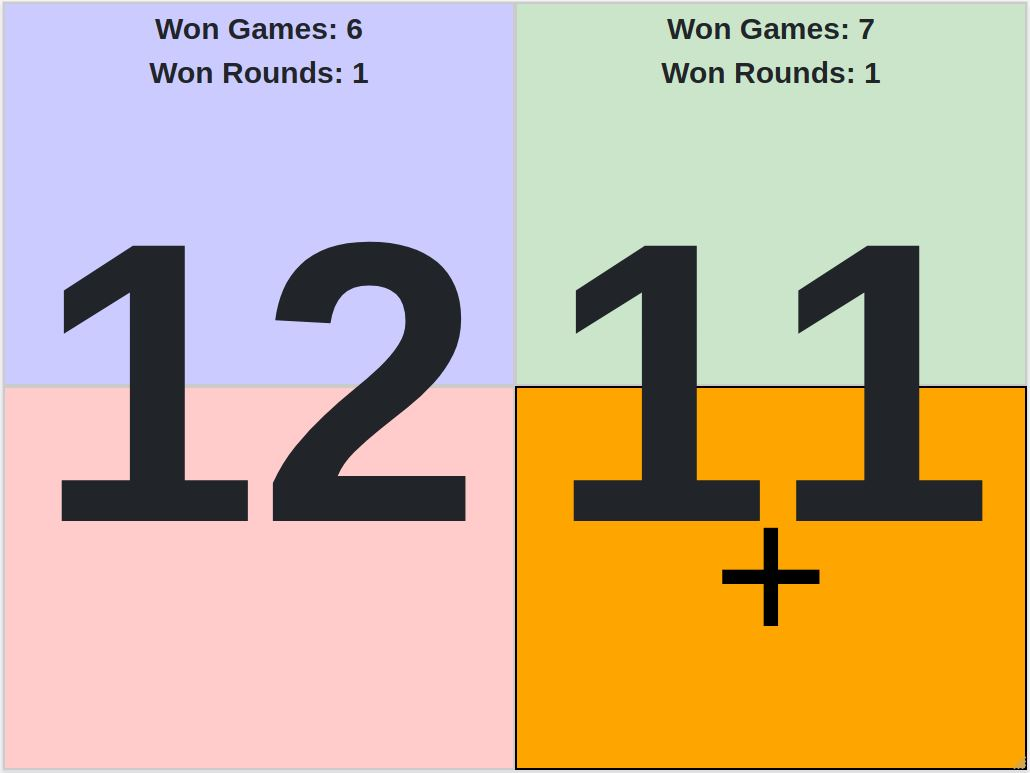
\includegraphics[scale=0.5]{Grafiken/game_seite}
\label{Game Seite}
\caption{Game-Seite der Benutzeroberfläche}
\end{figure}

In Abbildung \ref{Game Seite} ist die Game-Seite der Benutzeroberfläche dargestellt. Diese Seite stellt viele Informationen des Spiels des Benutzers dar. Die Seite ist in vier gleich große farbige Rechtecke aufgeteilt. Diese farbigen Rechtecke stellen die Position der Spieler auf dem Feld dar. Die Farben der Rechtecke entsprechen den Farben die der Benutzer für die Spieler gewählt hat. Eines der vier Rechtecke ist farbig hervorgehoben und mit einem Kreuz markiert. Dadurch wird gekennzeichnet, dass die Person, welche auf dieser Position steht, Aufschlag hat. Zusätzlich zu den Positionen der Spieler und der Aufschlaganzeige, werden die gewonnen Punkte, Sätze und Spiele des jeweiligen Teams auf der jeweiligen Seite des Spielfeldes angezeigt.

\section{Ergonomie}

\begin{quote}
	Ergonomie von IT-Systemen bedeutet die Verbesserung (Optimierung) deren Benutzbarkeit aufgrund objektiver und subjektiver Faktoren. Im wesentlichen zählen zu ergonomischen Faktoren die Benutzungsoberfläche, die Reaktivität (gefühlte Performance) sowie die Verfügbarkeit und Robustheit eines Systems.
\end{quote}

\section{Geschäftsregeln}

\begin{quote}
	Wie behandeln Sie Geschäftslogik oder Geschäftsregeln? Implementieren die beteiligten Fachklassen ihre Logik selbst, oder liegt die Logik in der Verantwortung einer zentralen Komponente? Setzen Sie eine Regelmaschine (rule-engine) zur Interpretation von Geschäftsregeln ein (Produktionsregelsysteme, forward- oder backward-chaining)?
\end{quote}

\section{Hochverfügbarkeit}

\begin{quote}
	Wie erreichen Sie hohe Verfügbarkeit des Systems? Legen Sie Teile redundant aus? Verteilen Sie das System auf unterschiedliche Rechner oder Rechenzentren? Betreiben Sie Standby-Systeme?
	Könnte in Zusammenhang zu Clusterung stehen.
\end{quote}

\section{Internationalisierung}

\begin{quote}
	Unterstützung für den Einsatz von Systemen in unterschiedlichen Ländern, Anpassung der Systeme an länderspezifische Merkmale. Bei der Internationalisierung (aufgrund der 18 Buchstaben zwischen I und n des englischen Internationalisation auch i18n genannt) geht es neben der Übersetzung von Aus- oder EIngabetexten auch um verwendete Zeichensätze, Orientierung von Schriften am Bildschirm und andere (äußerliche) Aspekte.
\end{quote}

\section{Kommunikation, Integration}

\begin{quote}
	Kommunikation: Übertragung von Daten zwischen System-Komponenten. Bezieht sich auf Kommunikation innerhalb eines Prozesses oder Adressraumes, zwischen unterschiedlichen Prozessen oder auch zwischen unterschiedlichen Rechnersystemen.
	Integration: Einbindung bestehender Systeme (in einen neuen Kontext). Auch bekannt als: (Legacy) Wrapper, Gateway, Enterprise Application Integration (EAI).
\end{quote}

\section{Konfiguration}

\begin{quote}
	Die Flexibilität von IT-Systemem wird unter anderem durch ihre Konfigurierbarkeit beeinflusst, die Möglichkeit, manche Entscheidungen hinsichtlich der Systemnutzung erst spät zu treffen. Konfiguration kann zu folgenden Zeitpunkten erfolgen:
	Während der Programmierung: Dabei werden beispielsweise Server-, Datei- oder Verzeichnisnamen direkt ("hart") in den Programmcode aufgenommen.
	Während des Deployments oder der Installation: Hier werden Konfigurationsinformationen für eine bestimmte Installation angegeben, etwa der Installationspfad.
	Beim Systemstart: Hier werden Informationen vor oder beim Programmstart dynamisch gelesen.
	Während des Programmablaufs: Konfigurationsinformation wird zur Programmlaufzeit erfragt oder gelesen.
\end{quote}

\section{Logging, Protokollierung}

\begin{quote}
	
	Es gibt zwei Ausprägungen der Protokollierung, das Logging und das Tracing . Bei beiden werden Funktions- oder Methodenaufrufe in das Programm aufgenommen, die zur Laufzeit über den Status des Programms Auskunft geben.
	In der Praxis gibt es zwischen Logging und Tracing allerdings sehr wohl Unterschiede:
	\begin{itemize}
		\item Logging kann fachliche oder technische Protokollierung sein, oder eine beliebige Kombination von beidem.
		\item Fachliche Protokolle werden gewöhnlich anwenderspezifisch aufbereitet und übersetzt. Sie dienen Endbenutzern, Administratoren oder Betreibern von Softwaresystemen und liefern Informationen über die vom Programm abgewickelten Geschäftsprozesse.
		\item Technische Protokolle sind Informationen für Betreiber oder Entwickler. Sie dienen der Fehlersuche sowie der Systemoptimierung.
		\item Tracing soll Debugging -Information für Entwickler oder Supportmitarbeiter liefern. Es dient primär zur Fehlersuche und -analyse.
	\end{itemize}
\end{quote}

\section{Management und Administrierbarkeit}

\begin{quote}
	Größere IT-Systeme laufen häufig in kontrollierten Ablaufumgebungen (Rechenzentren) unter der Kontrolle von Operatoren oder Administratoren ab. Diese Stakeholder benötigen einerseits spezifische Informationen über den Zustand der Programme zur Laufzeit, andererseits auch spezielle Eingriffs- oder Konfigurationsmöglichkeiten.
\end{quote}

\section{Migration}

\begin{quote}
	Für manche Systeme gibt es existierende Altsysteme, die durch die neuen Systeme abgelöst werden sollen. Denken Sie als Architekt rechtzeitig auch an alle organisatorischen und technischen Aspekte, die zur Einführung oder Migration der Architektur beachtet werden müssen.
	Beispiele:
	\begin{itemize}
		\item Konzept, Vorgehensweise oder Werkzeuge zur Datenübernahme und initialen Befüllung mit Daten
		\item Konzept zur Systemeinführung oder zeitweiliger Parallelbetrieb von Alt- und Neusystem
	\end{itemize}
	Müssen Sie bestehende Daten migrieren? Wie führen Sie die benötigten syntaktischen oder semantischern Transformationen durch?
\end{quote}

\section{Parallelisierung / Nebenläufigkeit}

\begin{quote}
	Programme können in parallelen Prozessen oder Threads ablaufen - was die Notwendigkeit von Synchronisationspunkten mit sich bringt. Die Grundlagen dieses Aspekten legt die Parallelverarbeitung. Für die Architektur und Implementierung nebenläufiger Systeme sind viele technische Detailaspekte zu berücksichtigen (Adressräume, Arten von Synchronisationsmechanismen (Guards, Wächter, Semaphore), Prozesse und Threads, Parallelität im Betriebssystem, Parallelität in virtuellen Maschinen und andere).
\end{quote}

\section{Persistenz}

\begin{quote}
	Persistenz (Dauerhaftigkeit, Beständigkeit) bedeutet, Daten aus dem (flüchtigen) Hauptspeicher auf ein beständiges Medium (und wieder zurück) zu bringen.
	Einige der Daten, die ein Software-System bearbeitet, müssen dauerhaft auf einem Speichermedium gespeichert oder von solchen Medien gelesen werden:
	\begin{itemize}
		\item Flüchtige Speichermedien (Hauptspeicher oder Cache) sind technisch nicht für dauerhafte Speicherung ausgelegt. Daten gehen verloren, wenn die entsprechende Hardware ausgeschaltet oder heruntergefahren wird.
		\item Die Menge der von kommerziellen Software-Systemen bearbeiteten Daten übersteigt üblicherweise die Kapazität des Hauptspeichers.
		\item Auf Festplatten, optischen Speichermedien oder Bändern sind oftmals große Mengen von Unternehmensdaten vorhanden, die eine beträchtliche Investition darstellen.
	\end{itemize}
	Persistenz ist ein technisch bedingtes Thema und trägt nichts zur eigentlichen Fachlichkeit eines Systems bei. Dennoch müssen Sie sich als Architekt mit dem Thema auseinander setzen, denn ein erheblicher Teil aller Software-Systeme benötigt einen effizienten Zugriff auf persistent gespeicherte Daten. Hierzu gehören praktisch sämtliche kommerziellen und viele technischen Systeme. Eingebettete Systeme (embedded systems ) gehorchen jedoch oft anderen Regeln hinsichtlich ihrer Datenverwaltung.
\end{quote}

\section{Plausibilisierung und Validierung}

\begin{quote}
	Wo und wie plausibilisieren und validieren Sie (Eingabe-)daten, etwa Benutzereingaben?
\end{quote}

\section{Sessionbehandlung}

\begin{quote}
	Eine Session, auch genannt Sitzung, bezeichnet eine stehende Verbindung eines Clients mit einem Server. Den Zustand dieser Sitzung gilt es zu erhalten, was insbesondere bei der Nutzung zustandsloser Protokolle (etwa HTTP) wichtige Bedeutung hat. Sessionbehandlung stellt für Intra-  und Internetsysteme eine kritische Herausforderung dar und beeinflusst häufig die Performance eines Systems.
\end{quote}

\section{Sicherheit}

\begin{quote}
	Die Sicherheit von IT-Systemen befasst sich mit Mechanismen zur Gewährleistung von Datensicherheit und Datenschutz sowie Verhinderung von Datenmissbrauch.
	Typische Fragestellungen sind:
	\begin{itemize}
		\item Wie können Daten auf dem Transport (beispielsweise über offene Netze wie das Internet) vor Missbrauch geschützt werden?
		\item Wie können Kommunikationspartner sich gegenseitig vertrauen?
		\item Wie können sich Kommunikationspartner eindeutig erkennen und vor falschen Kommunikationspartner schützen?
		\item Wie können Kommunikationspartner die Herkunft von Daten für sich beanspruchen (oder die Echtheit von Daten bestätigen)?
	\end{itemize}
	Das Thema IT-Sicherheit hat häufig Berührung zu juristischen Aspekten, teilweise sogar zu internationalem Recht.
\end{quote}

\section{Skalierung / Clusterung}

\begin{quote}
	Wie gestalten Sie Ihr System „wachstumsfähig“, so daß auch bei steigender Last oder steigenden Benutzerzahlen die Antwortzeiten und/oder Durchsatz erhalten bleiben?
\end{quote}

\section{Transaktionsbehandlung}

\begin{quote}
	Transaktionen sind Arbeitsschritte oder Abläufe, die entweder alle gemeinsam oder garnicht durchgeführt werden. Der Begriff stammt aus den Datenbanken - wichtiges Stichwort hier sind ACID-Transaktionen (atomar, consistent, isolated, durable). Im Bereich von NoSQL-Datenbanken gelten andere Kriterien.
\end{quote}

\section{Verteilung}

\begin{quote}
	Verteilung: Entwurf von Software-Systemen, deren Bestandteile auf unterschiedlichen und eventuell physikalisch getrennten Rechnersystemen ablaufen.
	Zur Verteilung gehören Dinge wie der Aufruf entfernter Methoden (remote procedure call, RPC), die Übertragung von Daten oder Dokumenten an verteilte Kommunikationspartner, die Wahl passender Interaktionsstile oder Nachrichtenaustauschmuster (etwa: synchron / asynchron, publish- subsribe, peer-to- peer).
\end{quote}